\documentclass[10pt,twocolumn,letterpaper]{article}

\usepackage{cvpr}
\usepackage{times}
\usepackage{epsfig}
\usepackage{graphicx}
\usepackage{amsmath}
\usepackage{amssymb}

% Include other packages here, before hyperref.

% If you comment hyperref and then uncomment it, you should delete
% egpaper.aux before re-running latex.  (Or just hit 'q' on the first latex
% run, let it finish, and you should be clear).
\usepackage[breaklinks=true,bookmarks=false]{hyperref}

\cvprfinalcopy % *** Uncomment this line for the final submission

\def\cvprPaperID{****} % *** Enter the CVPR Paper ID here
\def\httilde{\mbox{\tt\raisebox{-.5ex}{\symbol{126}}}}

% Pages are numbered in submission mode, and unnumbered in camera-ready
%\ifcvprfinal\pagestyle{empty}\fi
\setcounter{page}{4321}
\begin{document}

%%%%%%%%% TITLE
\title{CNN-based analysis of organoid growth}

\author{Shan Zhou \\
Facebook \\
\\
{\tt\small shanzhou@stanford.edu}
% For a paper whose authors are all at the same institution,
% omit the following lines up until the closing ``}''.
% Additional authors and addresses can be added with ``\and'',
% just like the second author.
% To save space, use either the email address or home page, not both
\and
Timothy Daley \\
Stanford University \\
Departments of Statistics and Bioengineering \\
{\tt\small tdaley@stanford.edu}
}

\maketitle
%\thispagestyle{empty}

%%%%%%%%% ABSTRACT
\begin{abstract}
High-throughput analysis of imaging data is critical for analysing large data typical of modern biological investigations.  Here we investigate a convolutional neural network-based approach to analyse the growth of organoids based off of imaging data.  
\end{abstract}

%%%%%%%%% BODY TEXT
\section{Introduction}

Predicting tumor growth rate is a first step in determining treatment options for cancer patients.  Fast growing tumors necessarily require more aggressive treatment.  It would be beneficial if patients could avoid aggressive treatments when possible.  

Alexandra Sockell of the Fordyce and Curtis labs in the Bioengineering and Genetics departments, respectively, of Stanford University has developed a microfluidic device to isolate single cells of a tumor and allow them to grow into organoids  within the microwell.  Organoids are three dimensional stem cell-like cultures that organize into a "mini-organ"~\cite{rios2018imaging}, and can be used to study cancer in a more natural environment than traditional cell lines~\cite{drost2018organoids}.
The objective of her research is to study the mechanisms of tumor growth by subjecting a large number of  individual cells to a wide range of treatments and conditions and track their condition by imaging.  She has taken 14 days of imaging over approximately 40 conditions.    For each day, there are approximate 200,000 well images across all conditions.  The number of cells per well is approximately Poisson, with most of the wells not containing any cells, 25\% have one cell, and smaller portion have more than 1.  We believe that the large number of images should provide a sufficient amount of data and information content to apply deep convolution neural network approach.  Our hypothesis is that the state of the cells in the early days should be related to their final state.  Therefore our objective to determine whether the early stages of the organoid can predict the growth rate and final state of the organoid.    



Previous approaches for high-throughput analysis of organoid imaging data did not look at single-cell microwell level data.  Instead they typically relied upon a large number of cells to quantify cell proliferation or death \cite{jabs2017screening},  used cell counting assays to calculate growth \cite{sebrell2018live}, or used single cell tracking to calculate cell motility \cite{geum2016epidermal}.  To our knowledge, no deep learning approaches have been proposed to analyse organoid imaging data, despite the large success in deep learning to analysing imaging data across a broad spectrum of applications.  We have found successful CNN approaches in related biological analysis such as high content screening \cite{simm2018repurposing}

\begin{figure}[b!]
\begin{center}
 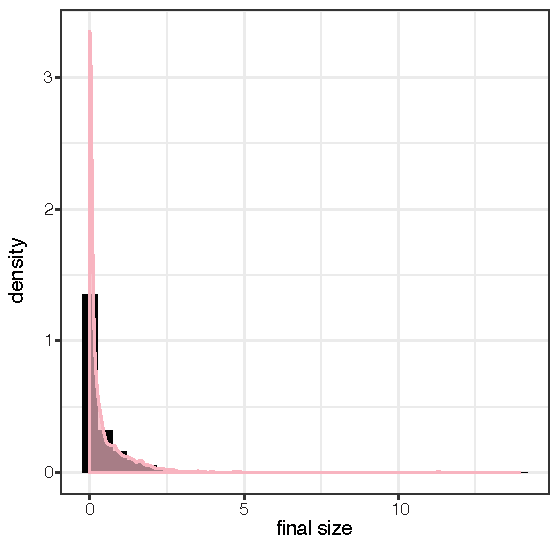
\includegraphics[width=0.8\linewidth]{figures/final_day_hyst2_area_density.pdf}
\end{center}
   \caption{Distribution of normalized final sizes.  There is a large peak at zero corresponding to empty wells or cells that died.}
\label{final_size_dist}
\end{figure}

\section{Data}

\begin{figure*}[t!]
\begin{center}
 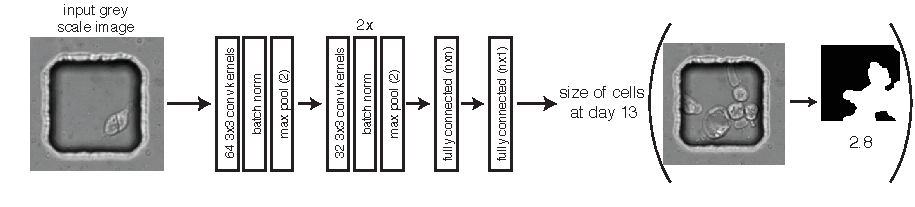
\includegraphics[width=0.8\linewidth]{figures/networkExampleImage.pdf}
\end{center}
   \caption{Example workflow of our algorithm.  The input is a 193$\times$193 greyscale image of the cell at day one.  We pass this through a convolutional neural network to predict the final size, normalized to have variance equal to 1.}
\label{workflow}
\end{figure*}

To achieve the goal of predicting tumor growth, we took the objective as predicting the final size of the tumor after 13 days of growth.  The final size is calculated by image segmentation of the interior of the microwell (Fig\ref{workflow}).  We normalized the sizes to have variance equal to one.  However, we did not mean center the data because we believe a final size equal to zero has meaning.  A final size equal to zero corresponds to either empty wells or cells that died.  





For input we took the day 1 images.  We determined that the day 0 images are not suffcient to predict  All images are black and white, so we converted them to greyscale and normalized the pixels to have zero mean and unit variance.  Our resulting images are 193$\times$193 with a single channel.   An example input image is show in figure~\ref{workflow}.







\section{Model}




To show the feasibility of a deep convolutional approach, we constructed a preliminary deep convolutional neural network. This network consisted of three convolutional layers, applying ReLu following each layer, followed by a single fully connected layer. We tried different kernel size, batch size, optimizers, and learning rates.  The performance across parameters was highly variable.  We found that the Adam optimizer with learning rate 1e$-4$ produce the best result for the preliminary models, and we present the results below for this learning rate.

As an initial test we use one hundred randomly selected images as a training set and another one hundred randomly selected images as a validation set.  Results are shown in Figure~\ref{results}.





\section{Preliminary Results}

Our preliminary results are poor.  Even for the small dataset of 100 images we can not achieve overfitting.  The mean square error at 50 epochs is equal to 0.2 (Figure \ref{results}\textbf{a}).  It may be that we can achieve zero error with sufficient training, but from this will almost certainly not generalize.     Most of the test set is predicted to be non-zero, but the true size is equal to zero (Figure \ref{results}\textbf{b}).  It may be that the labels are noisy, but recent work with training noisy labels indicates that this may not be a major problem~\cite{xue2019robust}.

To further test our ability to overtrain, we tried increasing the number of parameters by doubling the number of channels in each convolutional layer and adding a fully connected layer.  This resulted in $64 \cdot 5 \cdot 5 + 2 \cdot 32 \cdot 3 \cdot 3 + (193 \cdot 193 \cdot 32)^2 + 193 \cdot 193 \cdot 32 \approx \cdot 10^{12}$ parameters, while the number of total pixels is $100 \cdot 193 \cdot 193 \approx 4 \cdot 10^{6}$.  Therefore it should be very easy for this model to overfit and achieve zero training error.  Despite this we found that the training error plateaus at a mean square error of approximately $1.5$.  One hypothesis we have is that the large number of zeros in the final sizes ($\approx 47.5 \%$) makes it difficult for the neural network to properly train.  Instead, we find that sometimes the network tends to predict a constant value for almost all our data.  We may need to transfer our problem to a class prediction problem, where we are predicting whether the final size is zero or not based on the early images.  



\section{Future work}

We propose the following ideas to improve our results:
\begin{itemize}
\item Test out using later day images and several days in combination as input.  This may increase the information content of our input data.  In the latter case we would need to build a convolutional structure that will apply separate convolutions to each day, and combine the multiple days with fully connected layer.
\item Treat the problem as a classification problem.  We can try to predict whether the well at the final day is empty (final size $= 0$) or non-empty (final size $> 0$).  If we achieve good performance on this task, then we could take the non-empty well and retry the regression problem on only those wells.
\item Use a pre-trained model.  As a test we can use transfer learning to apply a pre-trained model on the images and test the performance.  This can also give a baseline for what we should expect for an upper bound of our error.
\end{itemize}

\begin{figure*}[t!]
\begin{center}
 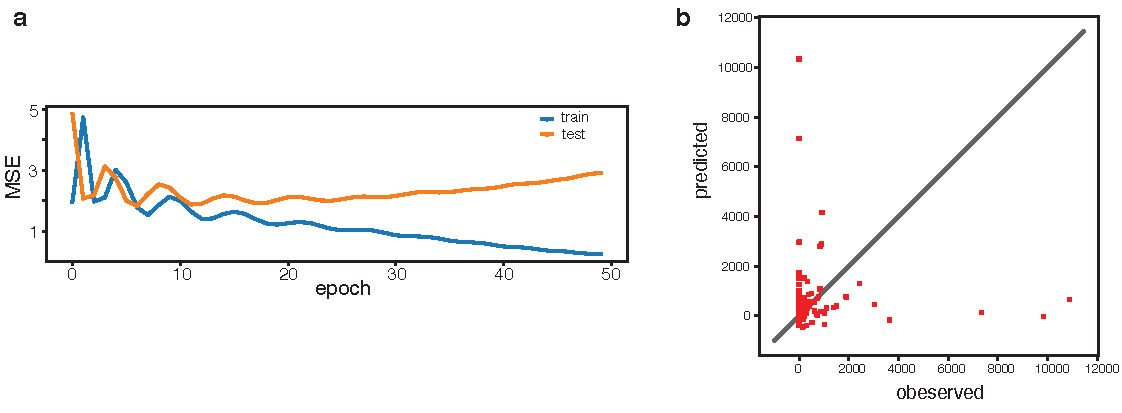
\includegraphics[width=0.8\linewidth]{figures/error_vs_epoch_and_validation_predictions_vs_observed_v2.pdf}
\end{center}
   \caption{\textbf{a} The training error (blue) and validation error (orange) as a function of training epoch.  \textbf{b} Predicted final size versus observed final size.}
\label{results}
\end{figure*}


We expect that changing the problem to a classification problem should help out tremendously.  First, this problem is much better established in the CNN community.  And second, since a large number of wells are empty, it should be easy for the CNN to identity and correctly classify these wells.    What would be interesting is identifying what characteristics of a live cell leads the model to classify it as likely to die.  We will first focus our efforts on this problem before moving to other strategies.  


{\small
\bibliographystyle{ieee}
\bibliography{bib}
}

\end{document}
